\documentclass[12pt]{scrartcl}

\usepackage[utf8]{inputenc}
\usepackage[T1]{fontenc}
\usepackage{lmodern}
\usepackage{graphicx}
%\usepackage[pdftex,hyperref,dvipsnames]{xcolor}
\usepackage{listings}
\usepackage[a4paper,lmargin={2cm},rmargin={2cm},tmargin={3.5cm},bmargin = {2.5cm},headheight = {4cm}]{geometry}
\usepackage{amsmath,amssymb,amstext,amsthm}
% \usepackage[lined,algonl,boxed]{algorithm2e} 
%\usepackage{algpseudocode}
\usepackage{tikz}
\usepackage{pgfplots}
\usepackage{url}
\usepackage{tcolorbox}
\usepackage[inline]{enumitem}
\usepackage[headsepline]{scrlayer-scrpage} 
\usepackage{float}

\usepackage[scale=0.55, lineVdist=1em]{secstack}
\pagestyle{scrheadings} 
\usetikzlibrary{automata,positioning}
\graphicspath{ {./images/} }

\usepgfplotslibrary{external}
%\tikzexternalize
\pgfplotsset{width=10cm,compat=1.9}
\pgfplotsset{every axis/.style={
    axis line style = thick,
    grid = both,
    tick pos = left,
    tick align = outside,
    tick style = {thick,black},
    fill = blue,
	line width = 2pt,
}}

\lstset{
  basicstyle=\ttfamily\small,
  numbers=left,
  numberstyle=\tiny,
  stepnumber=1,
  numbersep=8pt,
  frame=single,
  breaklines=true,
  columns=fullflexible
}

\lstset{
  language=C,
  basicstyle=\ttfamily\small,
  keywordstyle=\color{blue},
  commentstyle=\color{gray},
  stringstyle=\color{green!60!black},
  numbers=left,
  numberstyle=\tiny,
  stepnumber=1,
  numbersep=8pt,
  frame=single,
  breaklines=true,
  columns=fullflexible
}

\renewcommand{\theenumi}{(\alph{enumi})}
\renewcommand{\labelenumi}{\text{\theenumi}}
\renewcommand{\labelenumii}{(\roman{enumii})} 

\ohead{Marvin Simon (3883376)\\
       Jan Theil (3794698)}

\ihead{System and Web Security}

\newcounter{exnum}
\newcommand{\exercise}[1]{\section*{Problem \theexnum\stepcounter{exnum}: #1}}

\begin{document}

\setcounter{exnum}{2}
\exercise{Off-by-One Exploit}

For the attack string please see \textit{string1.c}.

This attack leverages the modification of the EBP. Like we can see in the attack screenshot, we are overwriting the Framepointer.

When the frame gets terminated with \texttt{leave} and \texttt{ret}, the processor is doing 3 things.
\begin{verbatim}
mov esp, ebp
\end{verbatim}
So the \textit{esp} now points to the address of the corrupted \textit{ebp} -> our buffer.
\begin{verbatim}
pop ebp
\end{verbatim}
Put the previous (or in our case mock) FramePointer into \textit{ebp} (e.g. AAAA).

And lastly...
\begin{verbatim}
pop eip
\end{verbatim}
Here our new return address which is saved in the buffer is loaded into the \textit{eip} and loads our shellcode.
\begin{figure}[H]
    \centering
    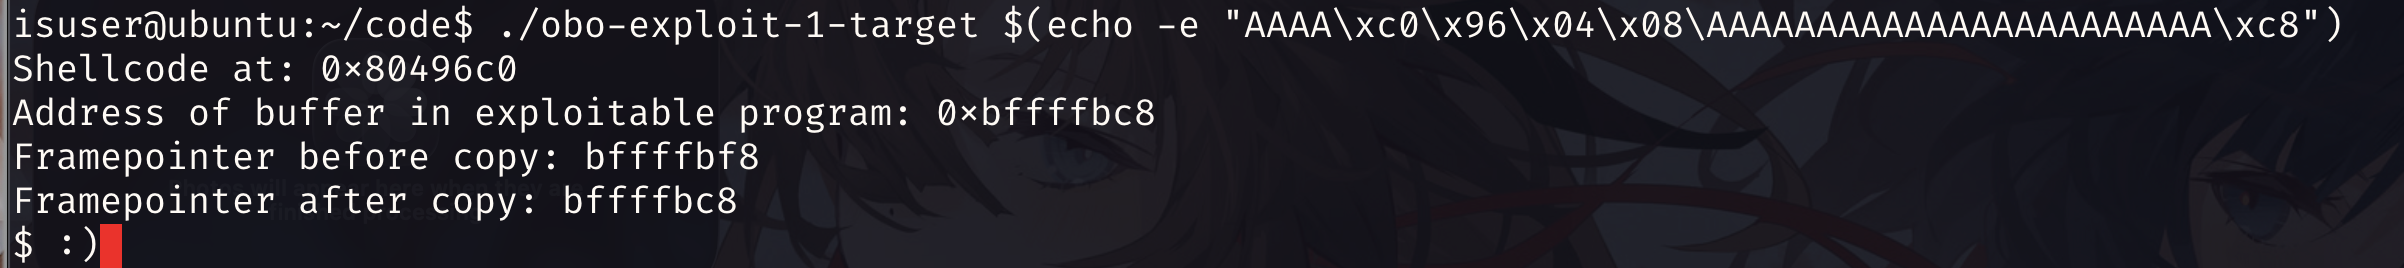
\includegraphics[width=\textwidth]{attack_2.png}
    \label{fig:attack2}
\end{figure}

The challenge of this exercise was to find the correct layout of the address and the understanding of how we can inject the return address into the construct.


\setcounter{exnum}{4}
\exercise{BSS-segment-based Overflow with Function Pointer}

For the source code please see \textit{attack4.c}.

The key idea is to overflow \texttt{buf} and overwrite the function pointer of \texttt{error\_handler} with the \texttt{system} function pointer.
\textit{attack4.c} creates a string and writes it into a file (see \textit{attack4.txt}). Calling \texttt{./bss-exploit-2-target \$(echo -e ’str’)}
with this string opens a shell.

\textit{attack4.c} works as follows:
\begin{itemize}
    \item Read the function pointer to \texttt{system} as argv. Here the pointer was \texttt{0x8048338}.
    \item Create a buffer that will overflow \texttt{buf}. In this case the buffer has to be at least $12 + 4 = 16$ bytes long.
    \item Write \texttt{"sh;"} to the beginning of this buffer and fill the rest with \texttt{"A"}s. This will open a shell and since it does not start with \texttt{'/'} the error handler will be called.
    \item Write the address to \texttt{system} in little endian format to the last 4 bytes of the buffer. This will be the new \texttt{error\_handler} pointer. 
\end{itemize}

The challenge of this exercise was to find a string that does not start with \texttt{'/'} but opens a shell. It should also not contain any \texttt{'\textbackslash 0'}s because that would
not overflow \texttt{buf}, since \texttt{strcpy} would not copy the whole string then. Hence, we are using \texttt{"sh;"} with filled up \texttt{"A"}s.

Running \texttt{./bss-exploit-2-target \$(echo -e '<attack4.txt>')} (see screenshot below or \textit{attack4.txt} for actual string) 
results in the shell being opened:

\begin{figure}[H]
    \centering
    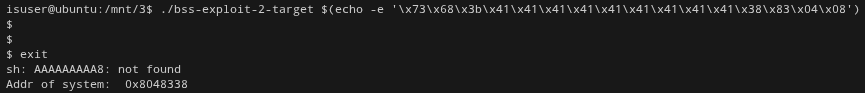
\includegraphics[width=\textwidth]{attack4.png}
    \label{fig:attack4}
\end{figure}

\end{document}
